\newpage

\chapter{Progress}

This section provides a comprehensive overview of the progress made by the project and the ongoing activities of the project. Below are the listed:

\begin{itemize}
    \item \textbf{Getting familiar with embedded systems:} Engaged in practical exercises from the Unphone: IoT book to build a foundational understanding of embedded systems. 
    \item \textbf{Getting familiar with Platform IO and MicroPython:} Currently getting familiar with the development environment and the programming language for effectively programming the Smart Patch.
    \item \textbf{Training}
    \begin{itemize}
        \item \textbf{iForge Training:} Completed iForge basic training and laser cut training. Will be finishing soldering training and 3D printing training by the end of December. 
        \item \textbf{Ethics Review Training:} Participated in ethics review training, ensuring that project activities aligned with ethical standards and guidelines.
    \end{itemize}
    \item \textbf{Scheduling Interviews:} In the process of scheduling interviews and preparing a list of questions to be asked in the interview. Coordinating with the interviewers to have the interviews sometime in January. 
    \item \textbf{Data Flow Diagram:} Developed a data flow diagram to visualize the movement and processing of information within the project, aiding in identifying key interactions and dependencies. Figure \ref{fig:data-flow-1} represents how data will be transmitted from an HCP to Smart patch and Figure \ref{fig:data-flow-2} represents how data collected by Smart patch will be transmitted to the dashboard in real-time. 
    
\begin{figure}
    \centering
    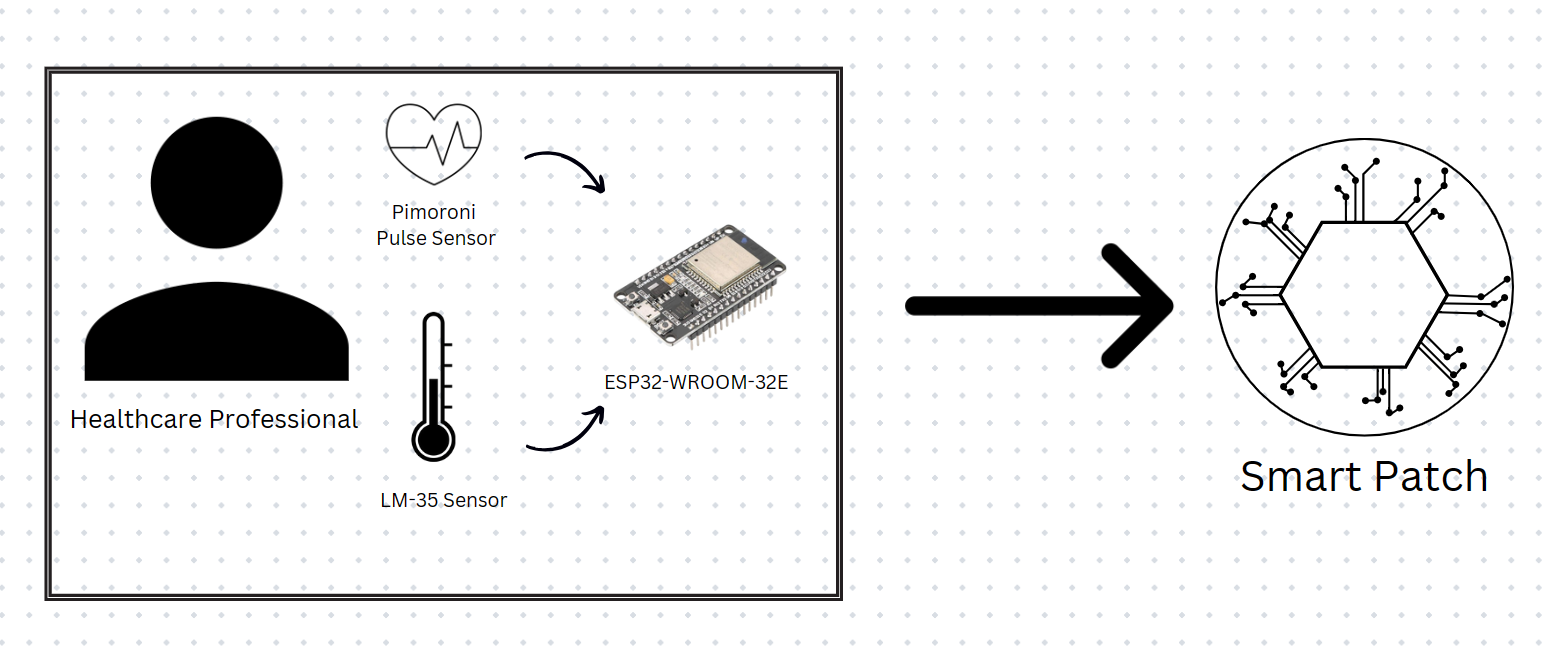
\includegraphics[width=\linewidth]{images/data-flow-1.png}
    \caption{Data Flow Diagram - 1 (From HCP to Smart Patch)}
    \label{fig:data-flow-1}
\end{figure}

\begin{figure}
    \centering
    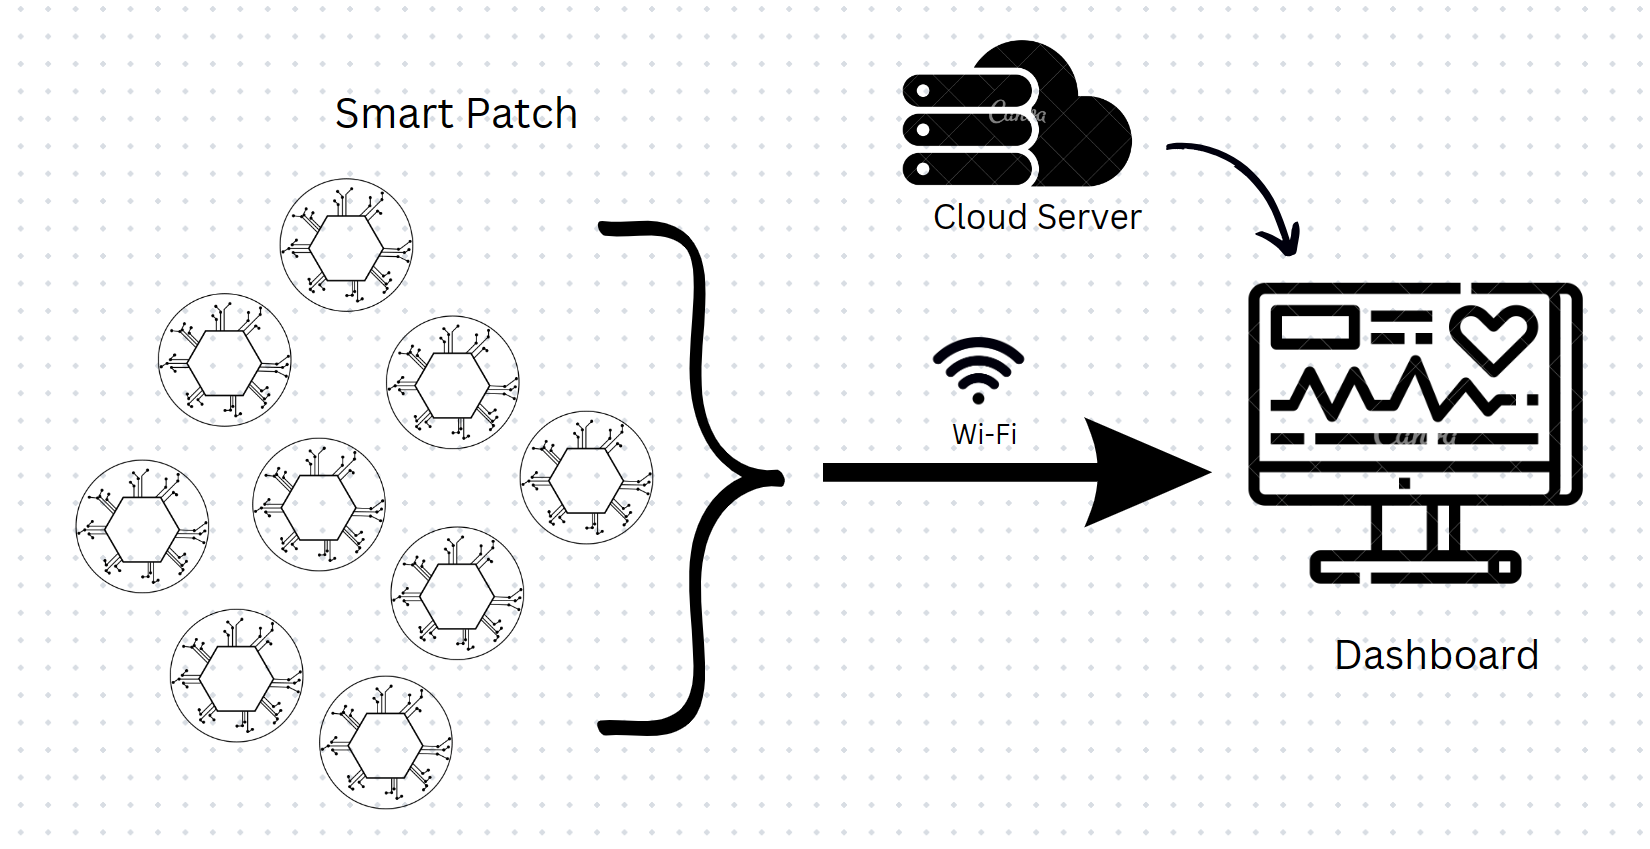
\includegraphics[width=\linewidth]{images/data-flow-2.png}
    \caption{Data Flow Diagram - 2 (From Smart Patch to Dashboard)}
    \label{fig:data-flow-2}
\end{figure}
    
    \item \textbf{Project Plan:} Established a comprehensive project plan using a Gantt Chart, providing a visual timeline of tasks and milestones to guide project execution and monitor progress. This project plan is laid out in Figure \ref{fig:gantt-chart}.

    \begin{figure}
        \centering
        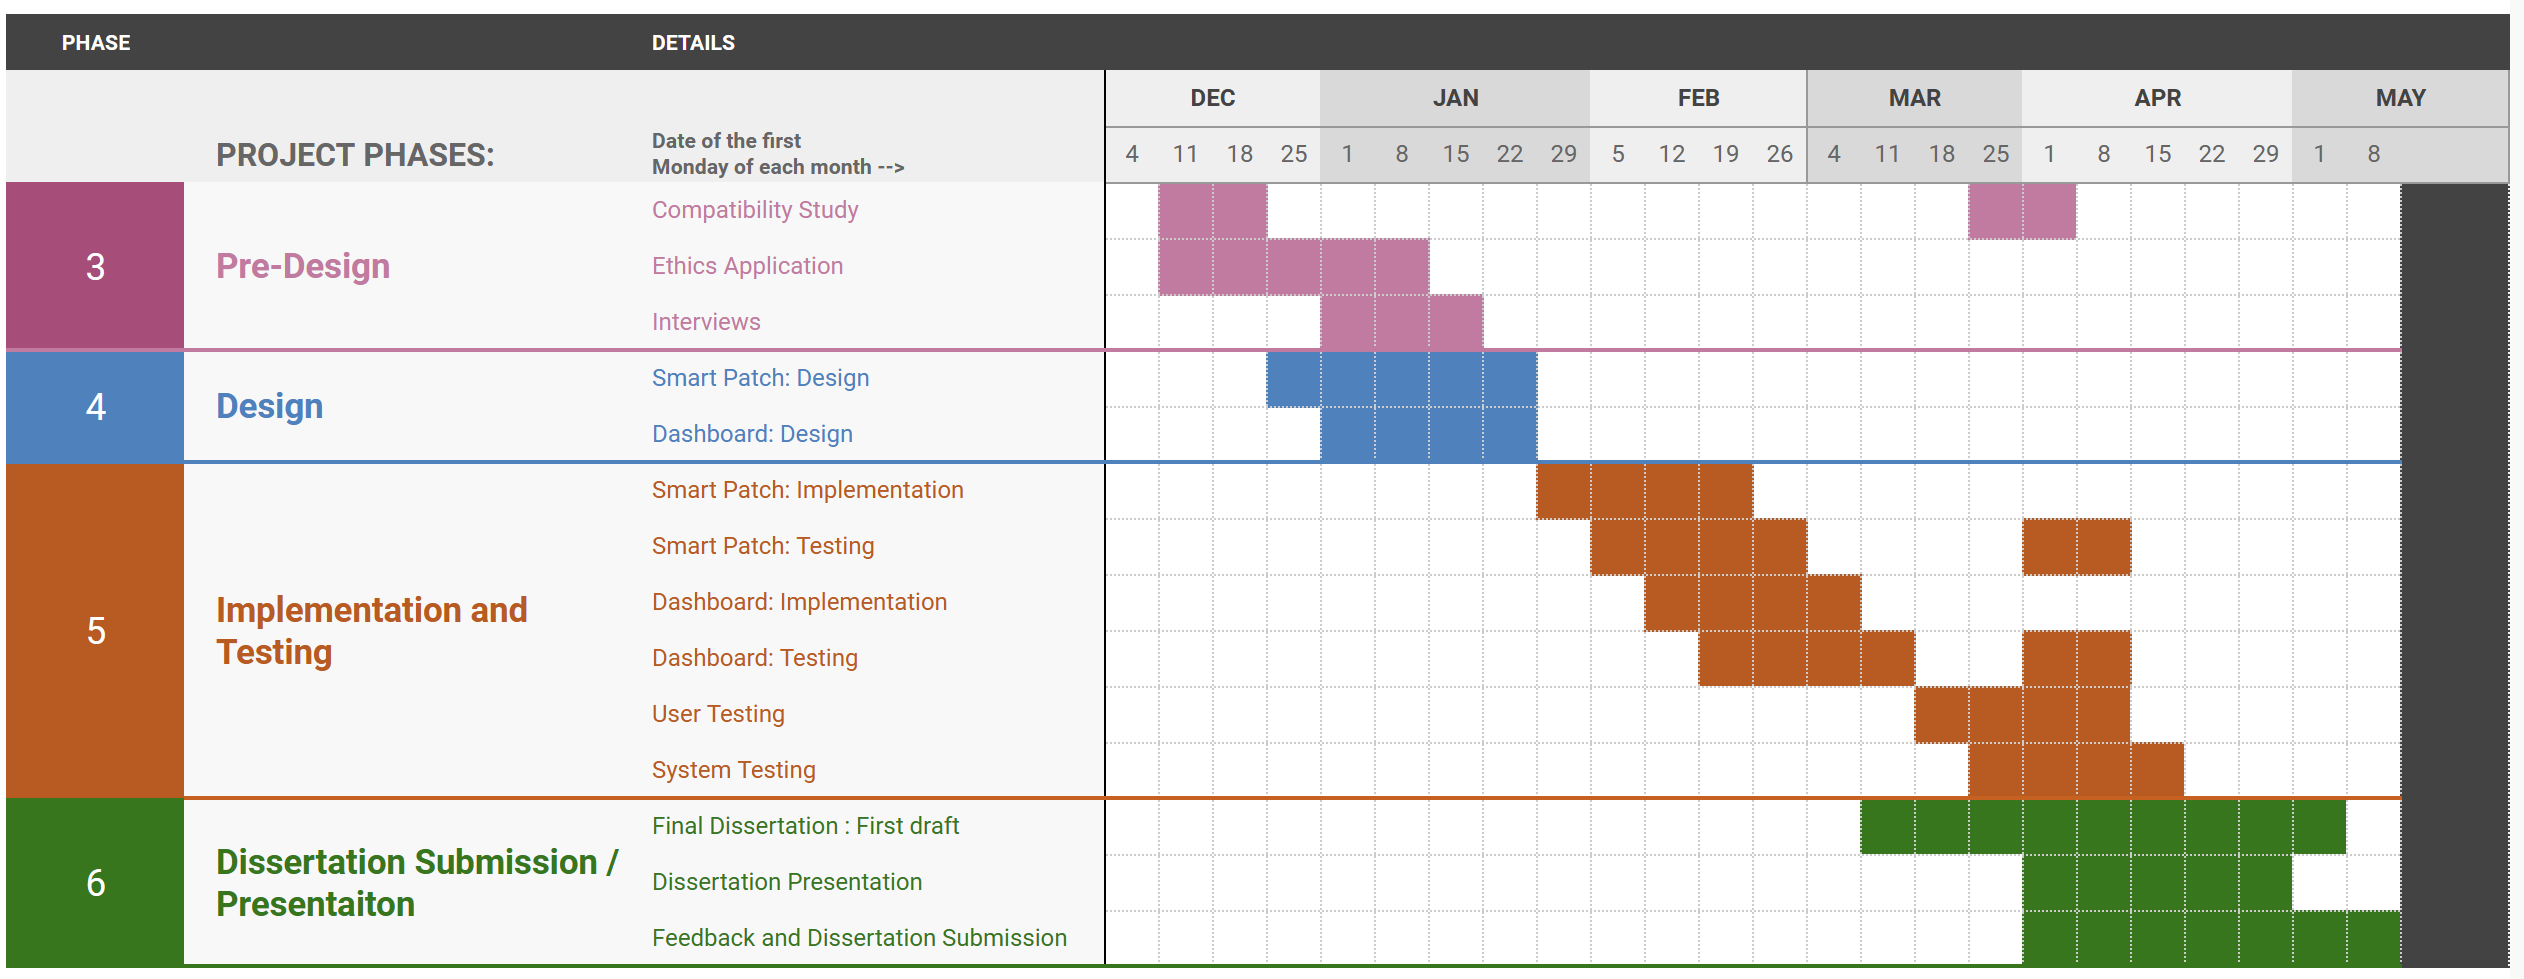
\includegraphics[width=1\linewidth]{images/gantt-chart.png}
        \caption{Project Plan }
        \label{fig:gantt-chart}
    \end{figure}
    
\end{itemize}








